\chapter{Тестирование и Отладка}

За счет разделения React приложений на компоненты, их очень удобно тестировать. Есть множество инструментов для создания тестов с React, и в этой главе мы разберем самые популярные из них, чтобы понять, какую выгоду мы можем из них извлечь.

\textbf{Jest} - тестовый фреймворк, который поддерживается силами \textit{Кристофером Пожером(Christopher Pojer)} из Facebook и членами сообщества; но ничто не мешает вам решить использовать \textbf{Mocha}. Мы посмотрим на оба способа создания лучшего тестового окружения.

Также вы узнаете о разнице между \textbf{Поверхностной отрисовкой (Shallow rendering)} и полной отрисовкой DOM с помощью \textbf{TestUtils} и \textbf{Enzyme}, как работает \textbf{Snapshot} тестирование и как собирать информацию о покрытии кода тестами.

После разбора самих инструментов мы перейдем к примеру покрытия тестами компонента из репозитория Redux и посмотрим на распространенные подходы, которые могут быть применены в сложных тестовых сценариях.

После разбора этой главы, вы сможете создать с нуля свое собственное тестовое окружение и написать тесты для компонентов вашего приложения.

В этой главе мы разберем следующие вопросы:

\begin{itemize}
	\item Почему важно покрывать приложение тесты, и как это ускоряет разработку
	\item Как настроить окружение с помощью Jest и начать писать тесты с TestUtils
	\item Как создать такое же тестовое окружение с Mocha
	\item Что такое Enzyme, и почему он рекомендуется для создания тестов React компонентов
	\item Как создать тесты для компонента из реального приложения
	\item Снимки (snapshots) Jest и процент покрытия с помощью библиотеки Istanbul
	\item Основные способы тестирования компонентов высшего порядка и сложных страниц с множеством дочерних компонентов
	\item Инструменты разработчика в React и подходы к обработке ошибок
\end{itemize}

\section{Польза от тестирования}

Тестирование web UI никогда не было простой задачей. Какие бы тесты мы не рассматривали, от модульных (unit) до сквозных (end-to-end), интерфейс всегда зависит от браузеров, взаимодействия с пользователем и множества других параметров, которые затрудняют создание оптимальной стратегии тестирования. 

Если вы когда-либо писали сквозные тесты, то должны знать, как трудно получить стабильно воспроизводимые результаты из-за различных факторов влияющих на выполнение тестов (например, нестабильность сети). Помимо этого, пользовательские интерфейсы часто обновляются, чтобы улучшить конверсию или просто добавить новые функции.

Если тесты становится сложно писать и поддерживать, у разработчиков пропадает мотивация в их создании. С другой стороны тесты очень важны, так как увеличивают доверие к коду, что увеличивает скорость и качество разработки. Если какая-то часть кода покрыта хорошими тестами, то разработчик, даже если вносит изменения, может быть уверен, что этот код работает корректно и готов к поставке. 

Часто разработчики могут быть сосредоточены над созданием новых возможностей для приложения, и в этот момент им может быть трудно понять, не ломают ли они уже существующий код. Наличие тестов может уберечь от регрессии приложения, так как их падение очень наглядно говорит о поломке в коде. Таким образом тесты добавляют уверенности в работоспособности кода и уменьшают время, необходимое для его релиза. 

Также тесты помогают улучшить качество кода в целом. Даже если обнаруживается какая-либо ошибка в приложении, ничто не мешает, не только исправить эту ошибку, но и создать специальный тест, который воспроизводит эту ошибку. Такой прием позволит в будущем быстрее обнаруживать появление ранее встречаемых ошибок.

К счастью, React упрощает написание тестов для UI. Тестирование отдельных компонентов (или деревьев компонентов) не так трудоемко, по сравнению с полным сквозным тестирование, особенно если компоненты обладают своей строго ограниченной областью ответственности.

А если компоненты не обладают внутренним состоянием, то они могут тестироваться как обычные функции.

Еще одна великолепная возможность, которую принесли современные инструменты, это возможность запускать тесты при помощи Node и консоли. Потребность в запуске браузера для проверки тестов значительно замедляет процесс разработки и ухудшает воспроизводимость тестов; что собственно и исправляется запуском тестов в консоли.

Когда компоненты тестируются только в консоли, могут всплыть неожиданные вещи при из запуске в браузере, но в общем и целом это происходит крайне редко.

Когда мы тестируем React компоненты, мы хотим быть уверены, что они работают корректно для различных комбинаций параметров, которые им можно передать. 

Также мы можем захотеть покрыть тестами различные состояния компонента, если таковые есть. Если состояние компонента меняется по нажатию на кнопку или какому-либо другому событию, то мы можем покрыть тестами обработчики событий, чтобы всегда быть уверенными, что они работают так, как должны работать.

После покрытия тестами основного функционала компонента, мы можем покрыть проверить \textbf{Пограничные случае (Edge cases)}. К пограничным случаям мы можем отнести ситуации, когда все параметры компонента приняли значение \textit{null}, или когда произошла какая-то ошибка. После того, как все тесты написаны, мы можем быть уверены в достаточной степени, что компонент ведет себя в соответствии с нашими ожиданиями.

Очень важно тестировать компоненты по отдельности, но это не гарантирует, что их совокупность также будет работать корректно. Как мы увидим далее, с React мы можем отрисовывать дерево элементов и тестировать взаимодействие компонентов внутри этого дерева. 

Есть различные подходы в написании тестов, но один из самых популярных - \textbf{Разработка через тестирование (Test Driven Development, TDD)}. Использование TDD подразумевает написание тестов перед написанием основного кода, за счет чего мы получаем возможность оценки корректности будущего кода до начала его разраотки. 

Следование этому подходу помогает писать код лучше, так как мы задумываемся о его дизайне еще до того, как начнем писать сам код, что обычно ведет к повышению качества.

\section{Тестирование JavaScript с Jest}

Лучший способ научиться тестировать React компоненты... это протестировать React компоненты. Поэтому в этой части мы попробуем написать небольшие компоненты и покрыть их тестами. 

Документация React говорит о том, что в Facebook для тестирования используется Jest. Но в общем случае ничто не запрещает вам использовать любой другой тестовый фреймворк.

А в следующей части вы научитесь тестировать компоненты при помощи Mocha.

Чтобы посмотреть, как работает Jest, мы создадим с нуля проект, установим все необходимые зависимости, и создадим компонент, который покроем тестами. Это будет весело!

Начнем с того, что создадим проект в пустой директории:

\begin{lstlisting}
	npm init
\end{lstlisting}

После того, как \textit{package.json} будет создан, мы можем начать устанавливать зависимости. Первой из них будет сам Jest:

\begin{lstlisting}
	npm install --save-dev jest
\end{lstlisting}

Для того, чтобы сказать npm, что мы хотим использовать команду \textit{jest} для запуска тестов, мы должны добавить соответствующую команду в файл \textit{package.json}:

\begin{lstlisting}
"scripts": {
  "test": "jest"
},
\end{lstlisting}

Для того, чтобы иметь возможность использовать все возможности ES2015 и JSX, мы должны установить Babel с соответствующими плагинами:

\begin{lstlisting}
    npm install --save-dev babel-jest babel-preset-es2015 babel-preset-react
\end{lstlisting}

Как вы уже можете догадаться, для конфигурации Babel нам понадобится файл \textit{.babelrc}, в котором мы укажем, какие пресеты мы хотим использовать в нашем проекте:

\begin{lstlisting}
{
  "presets": ["es2015", "react"]
}
\end{lstlisting}

Само собой нам потребуются React и ReactDom, чтобы иметь возможность создавать и запускать React компоненты:

\begin{lstlisting}
	npm install --save react react-dom
\end{lstlisting}

Настройка проекта закончена, мы можем запускать Jest для тестирования ES2015 и JSX кода, а также создавать и отрисовывать компоненты, но есть еще одна вещь, которую необходимо сделать.

Как мы уже сказали, мы хотим запускать тесты в консоли с Node. Но в этом случае мы не можем использовать ReactDOM, так как он требует DOM браузера.

Команда Facebook создала специальный инструмент, который называется \textit{TestUtils}. Этот инструмент позволяет без проблема тестировать React компоненты в любом тестовом фреймворке.

Давайте для начала его установим и посмотрим, какие возможности он предоставляет:

\begin{lstlisting}
	npm i --save-dev react-addons-test-utils
\end{lstlisting}

Теперь у нас есть все необходимое для тестирования компонентов. TestUtils позволяет выполнять поверхностную (shallow) отрисовку компонентов или отрисовывать компоненты в специальный DOM, отделенный от браузера. Также эта библиотека позволяет получать ссылки на компоненты, отрисованные в DOM, для проверки их состояния в целях тестирования.

Также с TestUtils возможно симулировать события браузера для проверки работоспособности обработчиков событий.

Давайте начнем с создания компонента, который в дальнейшем будет покрывать тестами.

Мы создадим компонент \textit{Button}, который будет получать из параметров текст и отрисовывать кнопку с этим текстом. Также в нем будет обработчик событий для этой кнопки. Для начала мы создадим только скелет этого компонента, а затем создадим к нему тесты, чтобы следовать подходу TDD.

Нам будет необходимо создать компонент класс, так как TestUtils на данный момент не умеет работать с функциональными компонентами.

Создадим файл \textit{button.js} и импортируем в нем React:

\begin{lstlisting}
import React from 'react'
\end{lstlisting}

Теперь мы можем определить сам компонент:

\begin{lstlisting}
class Button extends React.Component
\end{lstlisting}

В компоненте на данный момент будет только метод render, который будет возвращать пустой \textit{div}:

\begin{lstlisting}
render() {
  return <div />
}
\end{lstlisting}

И в конце добавим экспорт этого компонента:

\begin{lstlisting}
export default Button
\end{lstlisting}

Компонент подготовлен к покрытию тестами, теперь мы можем создать файл \textit{button.spec.js} и приступить к написанию тестов.

Jest ищет тесты во всех файлах, которые оканчиваются на \textit{.spec} и \textit{.test}, а также во всех файлах директории \textit{\_\_tests\_\_}; но вы можете изменить это поведение в настройках Jest, если этого требует ваш проект.

В начале файла \textit{button.spec.js} мы импортируем все необходимые зависимости:

\begin{lstlisting}
import React from 'react'
import TestUtils from 'react-addons-test-utils'
import Button from './button'
\end{lstlisting}

Нам нужен React, чтобы писать JSX код, TestUtils, на который мы посмотрим немного дальше, и только что созданный компонент\textit{Button}.

Для начала создадим простейший тест, чтобы убедиться, что система тестирования в принципе функционирует:

\begin{lstlisting}
test('works', () => {
  expect(true).toBe(true)
})
\end{lstlisting}

Функция \textit{test} принимает два параметра: описание теста и функцию с реализацией самого теста. Внутри мы используем функцию \textit{expect} для передачи Jest объекта, относительно которого мы хотим выполнить предсказание. Функция \textit{expect} возвращает объект с методами, которые позволяют конкретизировать предсказание. Например, функция \textit{toBe} проверяет, что переданный объект в точности соответствует заданному. 

Теперь мы можем выполнить в терминале команду:

\begin{lstlisting}
	npm test
\end{lstlisting}

Вы должны увидеть следующий результат:

\begin{lstlisting}
    PASS  ./button.spec.js
        works (3ms)
    Test Suites: 1 passed, 1 total
    Tests: 1 passed, 1 total
    Snapshots: 0 total
    Time: 1.48s
    Ran all test suites.
\end{lstlisting}

Если вы увидели в выводе в консоль слово PASS, вы готовы для создания реальных тестов.

Как мы уже сказали, с помощью тестов мы хотим убедиться, что компонент корректно обрабатывает полученные параметры, а обработчики событий выполняют свою работу.

Существует два основных способа тестировать React компонента:

\begin{itemize}
  \item Поверхностная отрисовка
  \item Монтирование компонентов в специальный DOM
\end{itemize}

Начнем с первого из них, так как он проще для понимания. При поверхностной отрисовке, как можно догадаться из названия, отрисовывается не все дерево компонентов, а только его верхняя часть \textit{высотой 1}, относительно которой мы можем выполнять различные проверки.

Отрисовка одного уровня дерева означает, что мы будет тестировать исходный компонент независимо от дочерних сколь сложны они бы не были. Таким образом, отрисовка дочерних компонентов не будет проводиться в принципе, поэтому они никак не смогут повлиять на результаты теста.

Первый тест, который мы можем сделать, это проверить, что переданный компоненту текст отрисовывается внутри кнопки.

Для начала создадим сам тест:

\begin{lstlisting}
test('renders with text', () => {
\end{lstlisting}

Создадим переменную с заданным текстом, которую мы будем передавать в параметры проверяемого компонента:

\begin{lstlisting}
const text = 'text'
\end{lstlisting}

И теперь можно выполнить поверхностную отрисовку компонента, для чего достаточно следующих трех строк:

\begin{lstlisting}
const renderer = TestUtils.createRenderer()
renderer.render(<Button text={text} />)
const button = renderer.getRenderOutput()
\end{lstlisting}

Сначала мы создаем \textit{renderer}, с помощью которого отрисовываем компонент \textit{Button}, и в последней строчке получаем результат отрисовки.

Результат отрисовки будет выглядеть примерно следующим образом:

\begin{lstlisting}
{
  '$$typeof': Symbol(react.element),
  type: 'button',
  key: null,
  ref: null,
  props: { onClick: undefined, children: 'text' },
  _owner: null,
  _store: {}
}
\end{lstlisting}

Если долго и пристально вглядываться, то можно увидеть в этом объекте React элемента. Его параметр \textit{props} отвечает за переданные элементу параметры, в том числе за дочерние (атрибут \textit{children}) элементы.

Теперь мы знаем, как выглядит результат отрисовки, а значит может легко проверить, что отрисовалась именно кнопка, а дочерним элементом является значение переменной \textit{text}:

\begin{lstlisting}
expect(button.type).toBe('button')
expect(button.props.children).toBe(text)
\end{lstlisting}

И не забудем в конце закрыть все скобки:

\begin{lstlisting}
})
\end{lstlisting}

Теперь, если вы запустите в консоли команду:

\begin{lstlisting}
	npm test
\end{lstlisting}

Вы должны увидеть что-то следующего вида:

\begin{lstlisting}
FAIL  ./button.spec.js
    renders with text
    expect(received).toBe(expected)
    Expected value to be (using ===):
      "button"
    Received:
      "div"
\end{lstlisting}

Тест упал, чего мы вообще говоря и ожидали, так как запустили тест для еще не реализованного компонента в соответствии с TDD подходом. Теперь мы можем вернуться к компоненту и поправить метод \textit{render} так, чтобы компонент проходил данный тест:

\begin{lstlisting}
render() {
  return (
    <button>
      {this.props.text}
    </button>
  )
}
\end{lstlisting}

Теперь при запуске тестов нас должна встретить зеленая галочка:

\begin{lstlisting}
PASS  ./button.spec.js
    renders with text (9ms)
    Test Suites: 1 passed, 1 total
    Tests:
    Snapshots:
    Time:
    Ran all test suites.
\end{lstlisting}

Поздравляю! Ваш первый тест для компонента, написанный в соответствии с TDD, выполнился успешно.

Теперь давайте посмотрим, как проверить, что компонент получил обработчик событий \textit{onClick}, и что этот обработчик вызывается при нажатии на кнопку.

Но перед тем, как мы начнем, нужно рассказать про две концепции: моки (mock) и открепленный (detached) DOM.

Первая упрощает проверку работы функций внутри теста. В данном тесте мы хотим передать компоненту функцию через параметр \textit{onClick} и проверить, что функция вызывается, когда происходит нажатие на кнопку.

Для того, чтобы сделать это, нам нужно создать специальную \textbf{мок (mock)} функцию (в других фреймворках такая функция может иметь другое название, например \textit{spy}). Такая функция работает как обыкновенная, но расширена дополнительными возможностями.Например, можно проверить, сколько раз и с какими параметрами была вызвана функция.

Для того, чтобы создать мок функцию при помощи Jest, мы можем использовать \textit{jest.fn()}.

Вторую концепцию нам нужно разобрать из-за того, что мы не можем симулировать события DOM с помощью \textit{TestUtils} при поверхностной отрисовке.

Это происходит из-за того, что для тестирования событий с \textit{TestUtils}, нам нужны реальные компоненты, а не React элементы.

Поэтому, для тестирования событий браузера, нам необходимо отрисовать наш компонент в открепленный DOM. Отрисовка компонента в полноценный DOM требует наличия браузера, но вместе с Jest идет специальный DOM, в который можно что-то отрисовать из консоли.

Отрисовка компонента в открепленный DOM несколько отличается от поверхностной отрисовки, поэтому давайте посмотрим, как это будет выглядеть в коде.

Для начала создадим новый тест:

\begin{lstlisting}
test('fires the onClick callback', () => {
\end{lstlisting} 

Создадим мок функцию \textit{onClick} при помощи Jest:

\begin{lstlisting}
const onClick = jest.fn()
\end{lstlisting}

Теперь мы отрисуем компонент в DOM полностью:

\begin{lstlisting}
const tree = TestUtils.renderIntoDocument(
  <Button onClick={onClick} />
)
\end{lstlisting}

Если мы распечатаем \textit{tree} в консоль, то увидим не React элемент, а полноценный компонент.

Из-за этого мы уже не можем просто проверить, что вернула функци \textit{renderIntoDocument}, но с помощью специального метода \textit{TestUtils} мы можем получить элемент кнопки, которая нас интересует:

\begin{lstlisting}
const button = TestUtils.findRenderedDOMComponentWithTag(
  tree,
  'button'
)
\end{lstlisting}

Как можно догадаться из названия функции, она ищет внутри дерева элемент с заданным тегом.

Теперь мы можем воспользоваться другим методом из \textit{TestUtils} для симуляции события:

\begin{lstlisting}
TestUtils.Simulate.click(button)
\end{lstlisting}

Объект \textit{Simulate} предоставляет функции, которые имеют названия, аналогичные названиям событий, и принимают один параметр для цели события.

И в конце выполняем проверку того, что функция была вызвана:

\begin{lstlisting}
expect(onClick).toBeCalled()
\end{lstlisting}

То есть мы просто проверяем, что \textit{мок} функция была вызвана.

Если мы снова запустим тесты, то увидим сообщение об ошибке, что ожидаемо, так как мы еще не реализовали работу функции \textit{onClick}:

\begin{lstlisting}
FAIL  ./button.spec.js
  fires the onClick callback
  expect(jest.fn()).toBeCalled()
  Expected mock function to have been called.
\end{lstlisting}

Именно так мы и работает при TDD подходе. Теперь вернемся в файл \textit{button.js} и реализуем обработчик событий:

\begin{lstlisting}
render() {
  return (
    <button onClick={this.props.onClick}>
      {this.props.text}
    </button>
  )
}
\end{lstlisting}

Теперь тесты должны показывать зеленый свет:

\begin{lstlisting}
PASS  ./button.spec.js
    renders with text (10ms)
    fires the onClick callback (17ms)
Test Suites: 1 passed, 1 total
Tests: 2 passed, 2 total
Snapshots: 0 total
Time: 1.401s, estimated 2s 
Ran all test suites.
\end{lstlisting}

Теперь наш компонент полностью протестирован и реализован в соответствии с написанными тестами.


\section{Гибкий тестовый фреймворк Mocha}

В этой части мы проделаем то же самое, чтобы показать, что вы можете использовать с React любой тестовый фреймворк по вашему желанию. Также будет полезным увидеть разницу между интегрированным фреймворком Jest, который старается все автоматизировать для более плавного использования (прим.пер. smooth developer experience что бы это не значило), и Mocha, который не делает никаких предположений относительно того, какие инструменты вам нужны. С Mocha вы можете установить любые библиотеки, которые вам нужны для тестирования React компонентов.

Для начала создадим новый npm проект в пустой директории:

\begin{lstlisting}
	npm init
\end{lstlisting}

И добавим саму библиотеку \textit{mocha}:

\begin{lstlisting}
	npm install --save-dev mocha
\end{lstlisting}

Так же как и для Jest, чтобы писать ES2015 код и JSX, нам потребуется Babel с парой плагинов:

\begin{lstlisting}
	npm install --save-dev babel-register babel-preset-es2015 babel-preset-react
\end{lstlisting}

Теперь, после установки Mocha и Babel, мы можем добавить скрипт для запуска тестов:

\begin{lstlisting}
"scripts": {
  "test": "mocha --compilers js:babel-register"
},	
\end{lstlisting}

Мы говорим \textit{npm}, что для выполнения команды \textit{test} необходимо запустить \textit{mocha} с флагом \textit{compilers} (для предварительного прогона исходного кода через \textit{Babel}).

Теперь добавим React и ReactDOM:

\begin{lstlisting}
	npm install --save react react-dom
\end{lstlisting}

А также \textit{TestUtils}, который позволяет нам отрисовывать компоненты в тестовом окружении:

\begin{lstlisting}
	npm install --save-dev react-addons-test-utils
\end{lstlisting}

Базовый инструментарий для работы с Mocha готов, но для того, чтобы привести все в соответствие с Jest, нам понадобится еще пара-тройка библиотек.

Первая из них - \textit{chai}, которая позволяет писать проверки в том же стиле, что и в Jest. Вторая - \textit{chai-spies}, с которой мы можем проводить шпионские операции для проверки функций, таких как \textit{onClick}. 

И последняя библиотека \textit{jsdom} позволяет нам создавать открепленный DOM, чтобы TestUtils могли отрисовывать компоненты без реального браузера:

\begin{lstlisting}
	npm install --save-dev chai chai-spies jsdom
\end{lstlisting}

Теперь мы готовы приступить к написанию тестов, для чего можем использовать созданный ранее файл \textit{button.js}. Мы уже реализовали компонент, поэтому мы не будем следовать TDD, но сейчас наша главная задача состоит в том, чтобы увидеть разницу между двумя тестовыми фреймворками.

Mocha ожидает, что тесты будут находиться в директории \textit{test}, поэтому мы можем создать ее и файл \textit{button.spec.js} внутри нее.

В начале файла импортируем все необходимые зависимости:

\begin{lstlisting}
import chai from 'chai'
import spies from 'chai-spies'
import { jsdom } from 'jsdom'
import React from 'react'
import TestUtils from 'react-addons-test-utils'
import Button from '../button'
\end{lstlisting}

Как вы можете заметить, после тестов с Jest, необходимо импортировать больше различных библиотек. Это связано с тем, что Mocha предоставляет вам самим выбрать, какие вспомогательные инструменты вам нужны.

Далее необходимо указать библиотеке \textit{chai} использовать \textit{spies}:

\begin{lstlisting}
chai.use(spies)
\end{lstlisting}

Сразу вытащим пару функция из \textit{chai}, которые потребуются нам далее в тестах:

\begin{lstlisting}
const { expect, spy } = chai
\end{lstlisting}

Далее мы создадим экземпляр \textit{jsdom} и установим его как DOM для отрисовки компонентов:

\begin{lstlisting}
global.document = jsdom('')
global.window = document.defaultView
\end{lstlisting}

И вот теперь мы можем создать первый тест. Обычно с Mocha (прим.пер. как и с Jest на самом деле) используется две функции для написания тестов: \textit{describe}, которая описывает набор тестов, и \textit{it}, внутри которой непосредственно описываются тесты.

В данном случае мы описываем поведение кнопки:

\begin{lstlisting}
describe('Button', () => {
\end{lstlisting}

И затем мы создаем первый тест, в котором проверяем, что у компонента правильные тип и текст:

\begin{lstlisting}
it('renders with text', () => {
\end{lstlisting}

Создадим переменную с текстом, которую будем использовать для проверки текста в кнопке:

\begin{lstlisting}
const text = 'text'
\end{lstlisting}

Далее сделаем поверхностную отрисовку компонента, как мы делали это до этого:

\begin{lstlisting}
const renderer = TestUtils.createRenderer()
renderer.render(<Button text={text} />)
const button = renderer.getRenderOutput()
\end{lstlisting}

И в конце выполним проверки:

\begin{lstlisting}
expect(button.type).to.equal('button')
expect(button.props.children).to.equal(text)
\end{lstlisting}

Как вы можете заметить, есть небольшие синтаксические различия. Вместо функциил \textit{toBe} появилась \textit{to.equal} из библиотеки \textit{chai}. Но результат одинаковый: сравнение двух значений.

Не забудем закрыть скобки для первого теста:

\begin{lstlisting}
})
\end{lstlisting}

В следующем тесте мы будем проверять, что вызывается функция обратного вызова \textit{onChange}:

\begin{lstlisting}
it('fires the onClick callback', () => {
\end{lstlisting}

Создадим мок функцию с помощью \textit{spy}, аналогично тому, как до этого создавали при помощи \textit{jest.fn}:

\begin{lstlisting}
const onClick = spy()
\end{lstlisting}

Отрисовываем компонент в открепленный DOM при помощи \textit{TestUtils}:

\begin{lstlisting}
const tree = TestUtils.renderIntoDocument(
  <Button onClick={onClick} />
)
\end{lstlisting}

А с помощью \textit{tree} мы можем найти нужный элемент в дереве:

\begin{lstlisting}
const button = TestUtils.findRenderedDOMComponentWithTag(
  tree,
  'button'
)
\end{lstlisting}

Следущий шаг - симуляция нажатия кнопки:

\begin{lstlisting}
TestUtils.Simulate.click(button)
\end{lstlisting}

И последним шагом можно проверить, была ли вызвана функция:

\begin{lstlisting}
expect(onClick).to.be.called()
\end{lstlisting}

И снова, хоть синтаксис немного и поменялся, но общая идея осталась той же, мы просто проверяем у функции, была ли она вызвана.

Теперь, если мы запустим \textit{npm test} в корневой директории, то увидим следующее сообщение:

\begin{lstlisting}
Button
	renders with text
	fires the onClick callback
	
2 passing (847ms)
\end{lstlisting}

Это означает, что наш тест выполнился успешно, а мы готовы использовать Mocha для тестирования наших компонентов.

\section{JavaScript инструменты для тестирования React}

На данный момент вы должны понимать, как тестировать компоненты при помощи Jest и Mocha, а также плюсы и минусы обоих подходов.

Также вы познакомились с TestUtils и узнали о двух способах отрисовки компонент: поверхностном и в открепленный DOM.

Однако вы могли заметить, что с TestUtils не всегда легко получить доступ к нужным элементам и их параметрам.

По этой причине разработчики из \textit{AirBnb} создали Enzyme, тестовый фреймворк, который работает поверх TestUtils и урощает работу с отрисованными компонентами.

API Enzyme приятно и схоже с jQuery, а также предоставляет удобные методы для работы с компонентами, их состоянием и параметрами.

Давайте посмотрим, как будут выглядеть уже написанные нами тесты, если мы перепишем их с Enzyme.

Давайте вернемся к проекту, где мы писали тесты с Jest, и добавим в него Enzyme:

\begin{lstlisting}
	npm install --save-dev enzyme
\end{lstlisting}

Теперь откроем файл \textit{button.spec.js} и поправим в нем импорты следующим образом:

\begin{lstlisting}
import React from 'react'
import { shallow } from 'enzyme'
import Button from './button'
\end{lstlisting}

Как вы можете увидеть, вместо \textit{TestUtils} мы импортируем \textit{shallow} из Enzyme. Из названия можно понять, что она выполняет поверхностную отрисовку компонента, но также обладает дополнительными возможностями.

Прежде всего, Enzyme позволяет эмулировать события даже при поверхностной отрисовке компонентов, чего мы не могли сделать с \textit{TestUtils}. И помимо этого, \textit{shallow} из Enzyme возвращает не просто React элемент, а \textbf{обертку (ShallowWrapper)} над ним, специальный объект с дополнительными параметрами и методами, которые мы разберем чуть дальше.

Давайте начнем с теста, который называется \textbf{renders with text}. Первая строка, где мы определяем переменную с текстом, остается той же самой:

\begin{lstlisting}
const text = 'text'
\end{lstlisting}

Поверхностная отрисовка компонента становится интуитивно понятнее и выразительнее. Три строки кода с использованием \textit{TestUtils} мы можем заменить одной:

\begin{lstlisting}
 const button = shallow(<Button text={text} />)
\end{lstlisting}

Объект \textit{button} представляет собой обертку над React элементом со вспомогательными методами, которые мы можем использовать для выполнения проверок:

\begin{lstlisting}
expect(button.type()).toBe('button')
expect(button.text()).toBe(text)
\end{lstlisting}

Теперь, вместо проверки параметров React элемента, названия которых могут измениться, мы используем библиотечные функции, которые абстрагируют внутри себя поиск нужных параметров (прим.пер. особенно если библиотека вовремя обновляется).

Функция \textit{type} проверяет тип элемента, а функиця \textit{text}, соответственно, текст внутри элемента. В нашем случае, это тот текст, который мы передали через параметры.

Теперь весь тест должен выглядеть следующим образом:

\begin{lstlisting}
test('renders with text', () => {
  const text = 'text'
  const button = shallow(<Button text={text} />)
  
  expect(button.type()).toBe('button')
  expect(button.text()).toBe(text)
})
\end{lstlisting}

Теперь тест выглядит лаконичнее и чище чем до этого.

Теперь поправим тест, который проверяет работу события \textit{onClick}. Снова, первая строчка остается той же:

\begin{lstlisting}
const onClick = jest.fn()
\end{lstlisting}

Мы можем также использовать мок функции из Jest для проверки срабатывания обработчиков событий.

Мы можем заменить строку, где мы использовали \textit{renderIntoDocument} для отрисовки компонента в открепленный DOM следующей:

\begin{lstlisting}
const button = shallow(<Button onClick={onClick} />)
\end{lstlisting}

Нам не нужно использовать \textit{findRenderedDOMComponentWithTag} для поиска кнопки, так как \textit{shallow} и так возвращает ссылку на нее.

Синтаксис для вызова эмуляции события немного отличается от \textit{TestUtils}, но все также интуитивно понятен:

\begin{lstlisting}
button.simulate('click')
\end{lstlisting}

У каждой обертки есть метод \textit{simulate}, который принимает имя события и допольнительные аргументы, которые в данном случае нам не нужны, но мы их разберем, когда будем разбираться с тестированием форм.

Проверка, была ли вызвана функция, остается той же:

\begin{lstlisting}
expect(onClick).toBeCalled()
\end{lstlisting}

Весь код теста выглядит следующим образом:

\begin{lstlisting}
test('fires the onClick callback', () => {
  const onClick = jest.fn()
  const button = shallow(<Button onClick={onClick} />)
  
  button.simulate('click')
  expect(onClick).toBeCalled()
})
\end{lstlisting}

Переход на Enzyme предельно прост, и при этом значительно улучшает читаемость кода.

Библиотека предоставляет множество полезных методом, таких как поиск вложенных элементов или поиск элементов по имени класса.

Есть методы для выполнения проверок параметров у компонентов, а также установка конкретных состояния или контекста.

Помимо поверхностной отрисовки, которой в случае Enzyme хватает для большинства случаем, библиотека предоставляет метод \textit{mount}, который отрисовывает компонент в DOM.


\section{Пример тестов из реального мира}

На данный момент мы разобрались, как настроить тестовое окружение и посмотрели на разные тестовые фреймворки. Пришло время посмотреть на тестирование компонентов из реального мира.

Компонент \textit{Button} из предыдущего примера был великолепен, и мы должны стремиться сохранять компоненты настолько простыми, насколько это возможно. Но порой нам приходится реализовывать какую-либо логику внутри компонентов, а также хранить состояние, что несколько усложняет задачу тестирования.

На этот раз мы собираемся протестировать компонент \textbf{TodoTextInput} из примера Redux \textbf{TodoMVC}:

\begin{lstlisting}
	https://github.com/reactjs/redux/blob/master/examples/todomvc/src/components/TodoTextInput.js
\end{lstlisting}

Вы можете скопировать его в ваш \textit{Jest} проект.

Это отличный пример для написания тестов, так как у компонента есть несколько параметров, его имя класса (прим.пер. я буду называть именем класса \textit{className} для CSS, чтобы не путать с ключевым словом \textit{class} JavaScript) меняется в соответствии с полученными параметрами, а также у него есть три обработчика с небольшим количеством логики, которую также стоит протестировать.

TodoMVC - пример создания \textit{стандартного} приложения при помощи различных фреймворков для их сравнения, что должно помочь разработчика в выборе между ними.

В результате у нас есть простенькое приложение, в котором можно добавлять задачи (to-do) и отмечать их выполнение. Для наших целей мы возьмем компонент, который отвечает за поле ввода для создания и редактирования задач. 

Имеет смысл, сначала пробежаться по коду самого компонента, чтобы понимать, что именно мы собираемся тестировать.

Начинается компонент с определения соответствующего ему класса:

\begin{lstlisting}
class TodoTextInput extends Component
\end{lstlisting}

В данном случае \textit{propTypes} определены при помощи свойства класса:

\begin{lstlisting}
static propTypes = {
  onSave: PropTypes.func.isRequired,
  text: PropTypes.string,
  placeholder: PropTypes.string,
  editing: PropTypes.bool,
  newTodo: PropTypes.bool
}
\end{lstlisting}

Для того, чтобы свойства класса поддерживались с Babel, необходимо добавить еще один плагин:

\begin{lstlisting}
	npm install --save-dev babel-plugin-transform-class-properties
\end{lstlisting}

И затем добавить этот плагин к остальным плагина в \textit{.babelrc}:

\begin{lstlisting}
"plugins": ["transform-class-properties"]
\end{lstlisting}

Состояние компонента также определено через свойство класса:

\begin{lstlisting}
state = {
  text: this.props.text || ''
}
\end{lstlisting}

Значение по умолчанию может быть пустой строкой или установлено из параметра \textit{text (this.props.test)}.

Далее идут три обработчика событий, каждый из которых представляет из себя стрелочную функцию (поэтому нет необходимости прикреплять их к экземплярам класса в конструкторе), которая также сохранена как свойство класса. 

Первый из них - обработчик окончания ввода (\textit{submit}):

\begin{lstlisting}
handleSubmit = e => {
  const text = e.target.value.trim()
  if (e.which === 13) {
    this.props.onSave(text)
    if (this.props.newTodo) {
      this.setState({ text: '' })
    }
  }
}
\end{lstlisting}

Функция получает объект события, проверяет, что была нажата клавиша \textit{Enter (13)}, убирает пробелы из введенной строки и сохраняет при помощи функции \textit{this.props.onSave}. Если параметр \textit{newTodo} - \textit{true}, то сбрасывает поле ввода для создания новой задачи.

Следующий обработчик будет отслеживать изменения в поле ввода:

\begin{lstlisting}
handleChange = e => {
  this.setState({ text: e.target.value })
}
\end{lstlisting}

Помимо того, что этот обработчик также определен через свойство класса, можно отметить, что оно сохраняет значение контролируемого поля ввода внутри состояния компонента.

И последний обработчик для отслеживания момента, когда пользователь убирает фокус с поля ввода (\textit{blur}):

\begin{lstlisting}
handleBlur = e => {
  if (!this.props.newTodo) {
    this.props.onSave(e.target.value)
  }
}
\end{lstlisting}

Он вызывает функцию \textit{onSave}, если значение параметра \textit{newTodo} равно \textit{false}.

И в конце находится метод \textit{render}, в котором определен элемент \textit{input} со всеми этими параметрами:

\begin{lstlisting}
render() {
  return (
    <input className={
      classnames({
        edit: this.props.editing,
        'new-todo': this.props.newTodo
      })}
      type="text"
      placeholder={this.props.placeholder}
      autoFocus="true"
      value={this.state.text}
      onBlur={this.handleBlur}
      onChange={this.handleChange}
      onKeyDown={this.handleSubmit} />
  )
}
\end{lstlisting}

Для применения нужного имени класса используется функция \textit{classnames}, которая создана \textit{Джедом Уотсоном (Jed Watson)} и удобна для расчета имени класса, которое зависит от различных логических выражений.

Также установлены несколько статических атрибутов (\textit{type} и \textit{autofocus}),	 через атрибут \textit{text} передается текст для управления значением поля ввода, и через соответствующие атрибуты переданы обработчики событий.

Перед тем, как начать, стоит понять, что именно мы собираемся тестировать и почему. Глядя на этот компонент, несложно выделить наиболее важные для покрытия тестами части. В данном случае, вы можете думать о данном компоненте как о коде, пришедшем в наследство от других команд (legacy code), или как о коде, который вы можете найти в новой компании.

Следущий список отражает функционал компонента, который в большей или меньшей степени подходит для покрытия тестами:

\begin{itemize}
  \item Состояние компонента проинициализировано значением, пришедшим в параметрах
  \item Параметр \textit{placeholder} корректно передается в поле ввода
  \item Применяется правильное имя класса
  \item Состояние компонента изменяется при вводе данных пользователем
  \item Функция \textit{onSave} вызывается корректно для различных состояний и условий
\end{itemize}

Пришло время начать писать код. Мы начнем с того, что создадим файл \textit{TodoTextInput.spec.js} со следующими импортами:

\begin{lstlisting}
import React from 'react'
import { shallow } from 'enzyme'
import TodoTextInput from './TodoTextInput'
\end{lstlisting}

Мы импортируем сам React, функцию \textit{shallow} из Enzyme и компонент, который будет тестировать. Также создадим функцию, которую будет передавать в параметр \textit{onSave} в некоторых тестах:

\begin{lstlisting}
const noop = () => {}
\end{lstlisting}

Теперь мы можем создать первый тест, в котором проверим, что значение по умолчанию устанавливается из полученных параметров:

\begin{lstlisting}
test('sets the text prop as value', () => {
  const text = 'text'
  const wrapper = shallow(
    <TodoTextInput text={text} onSave={noop} />
  )
  expect(wrapper.prop('value')).toBe(text)
})
\end{lstlisting}

Здесь все просто: создаем текстовую переменную, а затем выполняем поверхностную отрисовку компонента с передачей в него этой переменной. Также мы передаем функцию \textit{noop} в параметр \textit{onSave}, так как этот параметр является необходимым для компонента.

Далее мы выполняем проверку того, что значение в полученном элементе идентично значению переменной. Теперь, если мы запустим тест, то должны получить следующий результат:

\begin{lstlisting}
PASS  ./TodoTextInput.spec.js
  sets the text prop as value (10ms)
Test Suites:  1 passed, 1 total
Tests:        1 passed, 1 total
Snapshots:    0 total
Time:         1.384s
Ran all test suites.
\end{lstlisting}

Великолепно, продолжим писать тесты. Следующий тест будет очень похож на предыдущий за тем исключением, что мы будем проверять значение свойства \textit{placeholder}:

\begin{lstlisting}
test('uses the placeholder prop', () => {
  const placeholder = 'placeholder'
  const wrapper = shallow(
    <TodoTextInput placeholder={placeholder} onSave={noop} />
  )
  expect(wrapper.prop('placeholder')).toBe(placeholder)
})
\end{lstlisting}

Можно запустить тесты, оба должны светить зеленым светом.

Попробуем написать что-нибудь поинтереснее. Например, проверим, что имя класса меняется в соответствии полученным параметрам:

\begin{lstlisting}
test('applies the right class names', () => {
  const wrapper = shallow(
    <TodoTextInput editing newTodo onSave={noop} />
  )
  expect(wrapper.hasClass('edit new-todo')).toBe(true)
})
\end{lstlisting}

В этом тесте мы добавили компоненту два параметра (\textit{editing} и \textit{newTodo}), а затем проверили, что соответствующие классы добавились в имя класса.

Было бы лучше проверить каждый из классов отдельно, но идея должна быть понятна.

Следующий тест будет несколько сложнее, потому что теперь мы хотим проверить реакцию компонента на событие нажатия клавиши (key down).

Проверим, что при нажатии клавиши \textit{Enter}, вызывается функция \textit{onSave} с текущим значением поля ввода:

\begin{lstlisting}
test('fires onSave on enter', () => {
  const onSave = jest.fn()
  const value = 'value'
  const wrapper = shallow(<TodoTextInput onSave={onSave} />)
  
  wrapper.simulate('keydown', { target: { value }, which: 13 })
  
  expect(onSave).toHaveBeenCalledWith(value)
})
\end{lstlisting}

Сначала мы создаем мок функцию при помощи \textit{jest.fn()}, далее создаем переменную для установки значения поля ввода и отрисовываем компонент. После этого мы симулируем событие \textit{keydown} с кодом клавиши \textit{Enter (13)}.

У объекта события есть два параметра: \textit{target}, который отражает элемент, инициировавший событие, и \textit{which}, в котором находится код нажатой клавиши.

И в конце выполняем проверку, что функция \textit{onSave} была вызвана со значением поля ввода.

Теперь \textit{npm test} должен сказать, что 4 теста прошли успешно.

С помощью теста, похожего на предыдущий, мы можем проверить, что при нажатии отличной от \textit{Enter} клавиши функция \textit{onSave} не вызывается:

\begin{lstlisting}
test('does not fire onSave on key down', () => {
  const onSave = jest.fn()
  const wrapper = shallow(<TodoTextInput onSave={onSave} />)
  
  wrapper.simulate('keydown', { target: { value: '' } })
  
  expect(onSave).not.toBeCalled()
})
\end{lstlisting}

Тест очень похож на предыдущий за исключением выполняемый проверки, в которой на этот раз используется параметр \textit{.not}. Как можно догадаться, таким образом мы говорим, что ожидаем \textit{false} из вызова функции \textit{toBeCalled}.

Как вы могли заметить, синтаксис вызова проверок очень похож на разговорный язык.

У нас уже есть 5 зеленых тестов, двигаемся к следующему:

\begin{lstlisting}
test('clears the value after save if new', () => {
  const value = 'value'
  const wrapper = shallow(<TodoTextInput newTodo onSave={noop} />)
  
  wrapper.simulate('keydown', { target: { value }, which: 13 })
  
  expect(wrapper.prop('value')).toBe('')
})
\end{lstlisting}

Отличие на этот раз в том, что мы передали параметр \textit{newTodo}, который заставляет сбрасываться значение поля ввода по нажатию клавиши \textit{Enter}.

Следущий тест:

\begin{lstlisting}
test('updates the text on change', () => {
  const value = 'value'
  const wrapper = shallow(<TodoTextInput onSave={noop} />)
  
  wrapper.simulate('change', { target: { value } })
  
  expect(wrapper.prop('value')).toBe(value)
})
\end{lstlisting}

Этот тест проверяет, что контролируемое поле ввода работает корректно. Если в вашем приложение есть формы, то вам обязательно нужны такого рода тесты.

Мы симулируем событие \textit{change} со значением \textit{value}, а затем проверяем, что значение поля ввода изменилось соответствующим образом.

Теперь у нас есть 7 зеленых тестов, и остался только один.

В последнем тесте мы проверим, что событие \textit{blur} вызывает функцию обратного вызова только в том случае, если это не новый элемент:

\begin{lstlisting}
test('fires onSave on blur if not new', () => {
  const onSave = jest.fn()
  const value = 'value'
  const wrapper = shallow(<TodoTextInput onSave={onSave} />)
  
  wrapper.simulate('blur', { target: { value } })
  
  expect(onSave).toHaveBeenCalledWith(value)
})
\end{lstlisting}

Все как раньше: создали мок функцию, контрольное значение, вызвали событие \textit{blur}, проверили, что функция \textit{onSave} была вызвана с контрольным значением.

Если мы запустим тесты теперь, то должны увидеть чуть более объемистый вывод:

\begin{lstlisting}
PASS  ./TodoTextInput.spec.js
  sets the text prop as value (10ms)
  uses the placeholder prop (1ms)
  applies the right class names (1ms)
  fires onSave on enter (3ms)
  does not fire onSave on key down (1ms)
  clears the value after save if new (5ms)
  updates the text on change (1ms)
  fires onSave on blur if not new (2ms)
Test Suites:  1 passed, 1 total
Tests:        8 passed, 8 total
Snapshots:    0 total
Time:         2.271s
Ran all test suites.
\end{lstlisting}

Отличная работа, теперь компонент покрыт тестами. Теперь, если мы захотим изменить поведение компонента или добавить новые возможности, тесты покажут, где мы сломали старый функционал.

Это делает нас более уверенными в нашем коде, поэтому мы можем изменить любую строчку кода без страха, что сломаем старый функционал. 

\section{Snapshot-тестирование React компонентов}

После того, как вы увидели, как много тестов нужно написать для покрытия одного компонента, вы можете подумать, что на это будет уходить слишком много времени и в этом нет смысла.

Проверка всех комбинаций текста, значения поля ввода и имени класса довольно трудоемкий процесс, который требует написания большого количество кода. Однако, в большинстве случаев, для нас важно, что содержимое компонента не претерпит неожиданных изменений от изменений в коде. Для решения этой проблемы неплохо подходит \textbf{Snapshot-тестирование (Snapshot Testing)}.

Snapshot - это по сути \textit{снимок (picture)} компонента с определенными параметрами. Каждый раз, когда мы запускаем тесты, Jest создает снимок компонента и проверяет с эталонным на наличие изменений.

Содержимое снимка - это результат работы метода \textit{render} пакета \textit{react- test-renderer}, который необходимо установить:

\begin{lstlisting}
	npm install --save-dev react-test-renderer
\end{lstlisting}

После установки пакета, создадим новый файл \textit{TodoTextInput–snapshot.spec.js} со следующими импортами:

\begin{lstlisting}
import React from 'react'
import renderer from 'react-test-renderer'
import TodoTextInput from './TodoTextInput'
\end{lstlisting}

Импортируем React, чтобы использовать JSX, \textit{renderer}, чтобы создавать дерево для снимков, и компонент, который мы собираемся тестировать.

Теперь мы можем создать простенький тест:

\begin{lstlisting}
test('snapshots are awesome', () => {
\end{lstlisting}

В первой строке теста отрисуем компонент при помощи \textit{renderer}:

\begin{lstlisting}
const component = renderer.create(
  <TodoTextInput onSave={() => {}} />
)
\end{lstlisting}

В результате мы получаем экземпляр объекта, у которого есть специальный метод \textit{toJSON}. Вызовем этот метод следующей строкой:

\begin{lstlisting}
const tree = component.toJSON()
\end{lstlisting}

Таким образом мы получаем json со снимком элемента, который будет использоваться Jest для будущих сравнений.

Если мы распечатаем \textit{tree}, то получим примерно следующий результат:

\begin{lstlisting}
{ type: 'input',
    props:
      { className: '',
        type: 'text',
        placeholder: undefined,
        autoFocus: 'true',
        value: '',
        onBlur: [Function],
        onChange: [Function],
        onKeyDown: [Function] },
    children: null }
\end{lstlisting} 

И в конце выполняем проверку, что снимок соответствует сохраненному ранее:

\begin{lstlisting}
expect(tree).toMatchSnapshot()
\end{lstlisting}

После первого запуска \textit{npm test} снимок будет сохранен в директорию \textit{\_\_snapshots\_\_}.

Каждый файл в этой директории содержит снимок компонента. Если мы заглянем внутрь одного из таких файлов, то найдем вполне читаемое представление React компонента:

\begin{lstlisting}
exports[`test snapshots are awesome 1`] = `
<input
  autoFocus="true"
  className=""
  onBlur={[Function]}
  onChange={[Function]}
  onKeyDown={[Function]}
  placeholder={undefined}
  type="text"
  value="" />
`;
\end{lstlisting}

Теперь, если мы вернемся в тест и добавим параметр \textit{editing} в компонент, а затем запустим тест снова, то получим следующий результат:

\begin{lstlisting}
FAIL  ./TodoTextInput-snapshot.spec.js
        snapshots are awesome
        expect(value).toMatchSnapshot()
        Received value does not match stored snapshot 1.
        - Snapshot
        + Received
        @@ -1,8 +1,8 @@
         <input
           autoFocus="true"
        -  className=""
        +  className="edit"
           onBlur={[Function]}
           onChange={[Function]}
           onKeyDown={[Function]}
           placeholder={undefined}
           type="text"
\end{lstlisting}

Здесь мы можем увидеть, что текущий снимок отличается от сохраненного. В данном случае, в сохраненном снимке \textit{className} был пустым, а теперь содержит строку \textit{edit}.

Чуть ниже можно найти следующее сообщение:

\begin{lstlisting}
	Inspect your code changes or run with npm test -- -u to update them.
\end{lstlisting}

Снимками очень удобно пользоваться. Теперь, после обнаружения различий в сохраненном и полученном снимках, у вас есть два выбора: исправлять код или обновить сохраненные снимки, в последнем случае достаточно запустить команду: 

\begin{lstlisting}
	npm test -- -u
\end{lstlisting}

Как вы можете видеть, тестирование с помощью снимков значительно упрощает и ускоряет процесс написания тестов, так как можно проверять сразу весь компонент.


\section{Покрытие кода тестами}

Есть множество причин для написания тестов, и некоторые из них мы уже обсудили в предыдущей части. Но главной причиной остается повышение надежности кодовой базы.

По этой причине, я очень скептически отношусь к различным подсчетами количества тестов, количества строк кода или процента покрытия тестами. Я рекомендую не концентрироваться на численных показателях тестов, а думать об их реальной пользе.

Однако, в некоторых случаях имеет смысл отслеживать численные показатели покрытия тестами. В больших проектах, это может помочь находить файлы, которые протестированы недостаточно хорошо или не протестированы совсем.

Как уже говорилось, Jest предоставляет все возможности для запуска тестов, и конечно он предоставляет возможность собирать статистику о покрытии тестами кода.

Jest использует Istanbul, одну из самых популярных библиотек для подсчета покрытия кода тестами (если вы используете Mocha, вы можете установить ее вручную).

Для того, чтобы собрать статистику покрытия кода тестами с помощью Jest, достаточно добавить флаг \texttt{-{}-}coverage к \textit{npm test}. Также есть вариант, добавить блок с конфигурацией в \textit{package.json}, где установить флаг \textit{collectCoverage} в \textit{true}:

\begin{lstlisting}
"jest": {
  "collectCoverage": true
}
\end{lstlisting}

Если вы запустите тесты теперь, то увидите в консоли таблицу со статистикой покрытия кода тестами.

\begin{center}
  \makebox[\textwidth]{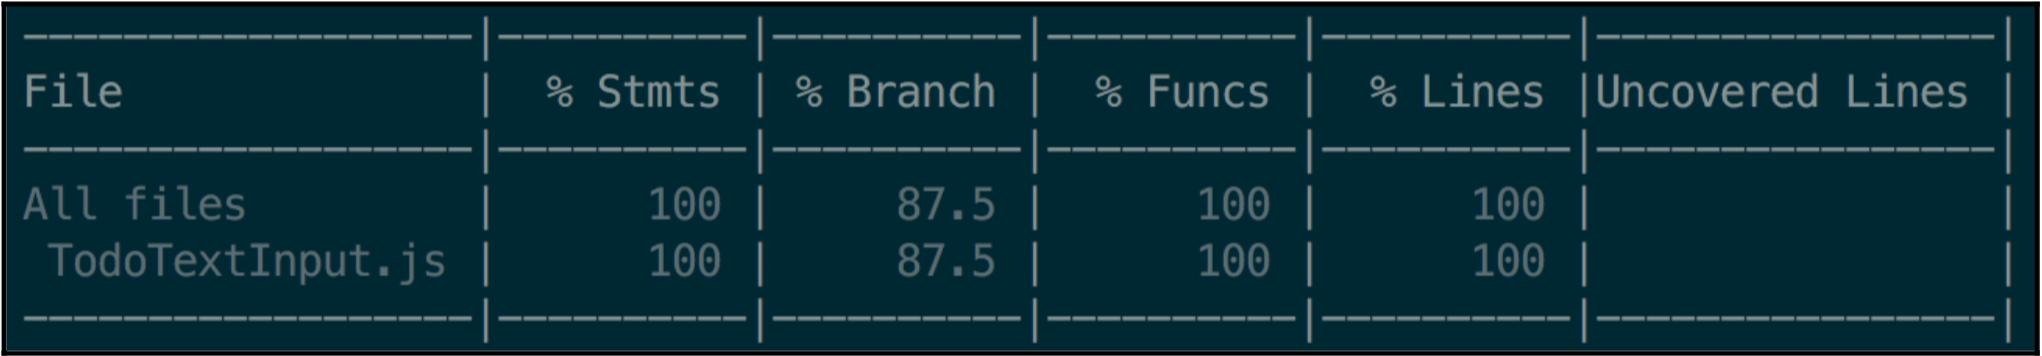
\includegraphics[width=0.6\paperwidth]{images/coverage}}
\end{center}

Как вы видите, наш файл практически полностью покрыт тестами. В первой колонке процент покрытых выражений, во второй условных переходов, в третьей протестированных функций и в четвертой строчек кода. И в последней колонке должны быть перечислены номера строк кода, которые еще не покрыты тестами, но в нашем случае таких нет. 

В наших тестах мы не достигли максимума только по критерию покрытия условных переходов. На самом деле я оставил один из них не протестированным специально, чтобы мы могли сделать это сейчас.

Если вы откроете файл \textit{TodoTextInput.js} и посмотрите в функцию \textit{onBlur}, вы найдете условный переход (хоть и без ветки \textit{else}):

\begin{lstlisting}
handleBlur = e => {
  if (!this.props.newTodo) {
    this.props.onSave(e.target.value)
  }
}
\end{lstlisting}

В случае, если это новая задача, функция \textit{onSave} вызываться не должна. 

А мы протестировали только тот случай, когда эта функция вызывается для существующей задачи. Но для того, чтобы убедиться, что все работает корректно, часто имеет смысл протестировать все возможные переходы.

Давайте откроем файл \textit{TodoTextInput.spec.js} и добавим еще один тест:

\begin{lstlisting}
test('does not fire onSave on blur if new', () => {
  const onSave = jest.fn()
  const wrapper = shallow(
    <TodoTextInput newTodo onSave={onSave} />
  )
  wrapper.simulate('blur')
  expect(onSave).not.toBeCalled()
})
\end{lstlisting}

Тест очень похож на предыдущий за тем исключением, что мы передаем параметр \textit{newTodo} и проверяем, что функцию \textit{onSave} не вызывается.

Теперь \textit{npm test} должен показывать 100\% покрытия по всем критериям.

\section{Распространенные подходы к созданию тестов}

В последней части главы о тестировании мы рассмотрим несколько распространенных шаблонов в тестировании React компонентов.

Вы уже познакомились с основами тестирования, однако иногда возникают ситуации, когда сложно понять, с какой стороны стоит начать тестирование кода. Это может произойти с \textbf{Компонентами высшего порядка (Higher-Order Components, HoC)}.


\subsection{Тестирование компонентов высшего порядка}

Как мы уже видели в предыдущих главах Компоненты высшего порядка предназначены для переиспользования кода между различными компонентами. HoC - это функция, которая принимает компонент и возвращает его с расширенным функционалом.

Тестирование таких компонентов может быть не так очевидно, как тестирование простых компонентов, поэтому имеет смысл разобрать пару распространенных решений вместе.

Попробуем протестировать HoC \textit{withData}, который мы создали в Главе 5. Единственный нюанс, мы немного поправим способ загрузки данных.

Функция \textit{withData} имеет следующую структуру:

\begin{lstlisting}
const withData = URL => Component => (...)
\end{lstlisting}

Эта функция принимает url, по которому необходимо загрузить данные, и передает загруженные данные компоненту. URL может быть функцией, которая получает параметры компонента, или строкой.

Функция \textit{withData} возвращает класс, определенный следующим способом:

\begin{lstlisting}
class extends React.Component
\end{lstlisting}

В конструкторе создается заготовка для скачиваемых данных:

\begin{lstlisting}
constructor(props) {
  super(props)
  
  this.state = { data: [] }
}
\end{lstlisting}

Данные загружаются в методе жизненного цикла \textit{componentDidMount}:

\begin{lstlisting}
componentDidMount() {
  const endpoint = typeof url === 'function'
    ? url(this.props)
    : url
  getJSON(endpoint).then(data => this.setState({ data }))
}
\end{lstlisting}

Как вы можете видеть, код немного отличается от того, что было в Главе 5: вместо использования \textit{fetch} мы используем \textit{getJSON}. Мы сделали это для того, чтобы вы увидели, как делать моки (mocks) для внешних модулей.

Это хорошая практика, оборачивать сторонние библиотеки и абстрактные API в отдельные модули, так как при тестировании это позволяет абстрагировать сам компонент от его зависимостей.

Функция \textit{getJSON} импортируется в начале файла:

\begin{lstlisting}
import getJSON from './get-json'
\end{lstlisting}

Эта функция возвращает промис (прим.пер. Promise; у меня рука не поднимется называть их обещ*ниями) на загрузку данных из сети.

И в методе \textit{render} мы отрисовываем компонент, передавая в него все параметры и текущее состояние:

\begin{lstlisting}
render() {
  return <Component {...this.props} {...this.state} />
}
\end{lstlisting}

Есть множество вещей, которые мы можем покрыть в данном случае тестами. Начнем с чего-то простого, например проверим, что параметры, полученные расширенным компонентом, корректно передаются целевому.

Затем мы можем проверить, что запрос отправляется на корректный адрес в обоих случаях: когда была передана строка с URL, или когда была передана функция для ее создания.

И самое главное, нужно проверить, что целевой компонент получает данные, которые возвращает функция \textit{getJSON}.

Создадим файл для тестов с необходимыми зависимостями:

\begin{lstlisting}
import React from 'react'
import { shallow, mount } from 'enzyme'
import withData from './with-data'
import getJSON from './get-json'
\end{lstlisting}

Мы импортируем и \textit{shallow} и \textit{mount} из Enzyme, так как для тестирования простых вещей нам не требуется полностью отрисованный DOM. Но как только мы собираемся использовать методы жизненного цикла компонентов, нам потребуется полная отрисовка.

Далее создадим пару вспомогательных переменных, которые пригодятся нам в тестах:

\begin{lstlisting}
const data = 'data'
const List = () => <div />
\end{lstlisting}

Первую из них мы будем использовать для проверки, что загруженные данные передаются целевому компоненту, а вторая будет минималистичным вариантом целевого компонента.

Создание почти пустого компонента для тестирования HoC распространенная практика, так как нам требуется компонент, который мы будем расширять. 

Далее следуем самая сложная часть данных тестов:

\begin{lstlisting}
jest.mock('./get-json', () => (
  jest.fn(() => ({ then: callback => callback(data) }))
))
\end{lstlisting}

Как уже было сказано, мы используем внешний модуль для загрузки данных. Одна из вещей, которую мы хотим избежать, это загрузка реальных данных; помимо этого мы не хотим, чтобы наши тесты начали падать, если сломается какая-либо из внешних библиотек. К счастью с помощью Jest очень удобно изолировать и подменять внешние зависимости для конкретного теста.

При помощи \textit{jest.mock} мы говорим Jest, что хотим заменить внешний модуль другой реализацией, которую должны передать вторым аргументом. В данном случае наша реализация содержит мок функцию \textit{jest.fn}, которая возвращает объект похожий на промис, но синхронный. У этого объекта есть метод \textit{then}, который получает функцию обратного вызова и вызывает ее с ранее созданными мок данными.

Начиная с этого момента мы можем тестировать наш HoC без опасений, что внешний модуль может повлиять на результат работы тестов.

Теперь мы можем приступить к созданию самих тестов. В первом из них проверим, что параметры, которые получает HoC, корректно передаются целевому компоненту:

\begin{lstlisting}
test('passes the props to the component', () => {
  const ListWithGists = withData()(List)
  const username = 'gaearon'
  
  const wrapper = shallow(<ListWithGists username={username} />)
  
  expect(wrapper.prop('username')).toBe(username)
})
\end{lstlisting}

Все должно быть понятно, но давайте вместе посмотрим на этот код. 
Сначала, мы создаем компонент \textit{ListWithGists} посредством расширения компонента \textit{List} с HoC \textit{withData}. Затем мы создаем переменную \textit{username}, которую будем передавать как параметр компоненту \textit{ListWithGists}, и выполняем поверхностную отрисовку. 

И в конце мы проверяем, что у отрисованного элемента есть параметр \textit{username} и он совпадает с заданным. Можно запустить \textit{npm test} и убедиться, что тест показывает зеленый свет.

Дальше наши тесты будут требовать отрисовки компонента в DOM. 
Сначала проверим, что передача строки с URL и функции для ее получения работают корректно. Начнем со статической строки:

\begin{lstlisting}
test('uses the string url', () => {
  const url = 'https://api.github.com/users/gaearon/gists'
  const withGists = withData(url)
  const ListWithGists = withGists(List)
  
  mount(<ListWithGists />)
  
  expect(getJSON).toHaveBeenCalledWith(url)
})	
\end{lstlisting}

В данном случае мы определили URL, а затем с помощью частичного применения создали новую функцию, которую дальше используем для расширения компонента \textit{List}.

Затем мы монтируем данный компонент в DOM и проверяем, что функция \textit{getJSON} была вызвана с заданным URL. 

Теперь проверим, что работает вызов функции для получения url:

\begin{lstlisting}
test('uses the function url', () => {
  const url = jest.fn(props => (
    `https://api.github.com/users/${props.username}/gists`
  )
  const withGists = withData(url)
  const ListWithGists = withGists(List)
  const props = { username: 'gaearon' }
  
  mount(<ListWithGists {...props} />)
  
  expect(url).toHaveBeenCalledWith(props)
  expect(getJSON).toHaveBeenCalledWith(
    'https://api.github.com/users/gaearon/gists'
  )
})
\end{lstlisting}

Сначала мы создаем мок функцию (что позволит проверить факт вызова), которая возвращает url. Создаем компонент \textit{ListWithGists}, расширяющий компонент \textit{List}, и параметры для этого компонента. 

Затем мы делаем две проверки:

\begin{itemize}
  \item В первой проверяем, что функция для создания url была вызвана с заданными аргументами
  \item И во второй проверяем, что функция \textit{getJSON} была вызвана с правильным адрессом
\end{itemize}

И в последнем тесте проверим, что то, что возвращает функция \textit{getJSON}, передается целевому компоненту:

\begin{lstlisting}
test('passes the data to the component', () => {
  const ListWithGists = withData()(List)
  
  const wrapper = mount(<ListWithGists />)
  
  expect(wrapper.prop('data')).toEqual(data)
})
\end{lstlisting}

Как всегда создаем расширенную версию компонента \textit{List} и монтируем его к DOM. Затем мы ищем компонент \textit{List} в том, что отрисовалось (прим.пер. в коде выше этого нет, постараться не забыть, сверить с кодом на api.github.com), и проверяем, что он получил параметр \textit{data} со значением, которое возвращает мок функция.

Если мы запустим \textit{npm test}, то должны увидеть, что все 4 теста проходят успешно.

Вот мы и разобрались, как можно тестировать компоненты высшего порядка в Jest и как изолировать наши тесты от внешних зависимостей.

\subsection{Паттерн Page Object}

Давайте посмотрим на еще один распространенный способ тестирования компонентов, который пригодится в тех случаях, когда дерево компонентов становится сложнее и появляется множество вложенных дочерних элементов.

В этих целях воспользуемся формой (Controlled form), созданной в Главе 6Ж

\begin{lstlisting}
class Controlled extends React.Component
\end{lstlisting}

Для начала вспомним, что этот компонент из себя представляет, а затем поговорим о его тестировании.

В конструкторе мы инициализируем начальное состояние и привязываем обработчики событий к экземпляру класса:

\begin{lstlisting}
constructor(props) {
  super(props)
  
  this.state = {
    firstName: 'Dan',
    lastName: 'Abramov',
  }
  
  this.handleChange = this.handleChange.bind(this)
  this.handleSubmit = this.handleSubmit.bind(this)
}
\end{lstlisting}

Обработчик \textit{handleChange} обновляет состояние при вводе данных:

\begin{lstlisting}
handleChange({ target }) {
  this.setState({
    [target.name]: target.value,
  })
}
\end{lstlisting}

Далее идет обработчик \textit{handleSubmit}, в котором сначала вызывается функция \textit{preventDefault} (чтобы браузер не выполнял никаких действий по отправке формы), а затем вызывается функция из параметров \textit{onSubmit}, в которую передаются введенные данные.

Этой функции не было в предыдущей реализации, но мы добавим ее, чтобы показать, как правильно тестировать такой компонент:

\begin{lstlisting}
handleSubmit(e) {
  e.preventDefault()
  
  this.props.onSubmit(
    `${this.state.firstName} ${this.state.lastName}`
  )
}
\end{lstlisting}

И в конце идет метод \textit{render}, в котором отрисовываются все поля ввода с нужными обработчиками событий:

\begin{lstlisting}
render() {
  return (
    <form onSubmit={this.handleSubmit}>
      <input
        type="text"
        name="firstName"
        value={this.state.firstName}
        onChange={this.handleChange}
      />
      <input
        type="text"
        name="lastName"
        value={this.state.lastName}
        onChange={this.handleChange}
      />
      <button>Submit</button>
    </form>
  )
}
\end{lstlisting}

Основной сценарий, который видится логичным для тестирования, это ввод каких-либо данных в форму, отправка (submit) формы и проверка, что функция \textit{onSumbit} вызвалась с нужными параметрами.

Вы уже должны представлять, как реализовать такой тестовый сценарий с помощью Enzyme, поэтому давайте быстро пройдем по реализации:

\begin{lstlisting}
test('submits the form', () => {
\end{lstlisting}

Прежде всего создадим мок функцию \textit{onSubmit}. Затем смонтируем компонент и получим ссылку на его обертку:

\begin{lstlisting}
const onSubmit = jest.fn()
const wrapper = shallow(<Controlled onSubmit={onSubmit} />)
\end{lstlisting}

Далее с помощью полученной ссылки найдем поле ввода и вызовем для него \textit{change} событие, для обновления его значения:

\begin{lstlisting}
const firstName = wrapper.find('[name="firstName"]')
firstName.simulate(
  'change',
  { target: { name: 'firstName', value: 'Christopher' } }
)
\end{lstlisting}

Проделаем то же самое со вторым полем ввода:

\begin{lstlisting}
const lastName = wrapper.find('[name="lastName"]')
lastName.simulate(
  'change',
  { target: { name: 'lastName', value: 'Chedeau' } }
)
\end{lstlisting}

После обновления полей ввода можно вызвать событие \textit{submit} на саму форму:

\begin{lstlisting}
const form = wrapper.find('form')
form.simulate('submit', { preventDefault: () => {} })
\end{lstlisting}

И затем проверить, что мок функция была вызвана с нужным значением:

\begin{lstlisting}
expect(onSubmit).toHaveBeenCalledWith('Christopher Chedeau')
\end{lstlisting}

И не забудем закрыть блок с тестом:

\begin{lstlisting}
})
\end{lstlisting}

Можно запустить \textit{npm test} и убедится, что он проходит. В общем и целом тест работает, но если мы посмотрим на него чуть пристальнее, то сможем обнаружить потенциальные проблемы.

Прежде всего бросается в глаза то, что код для заполнения полей в значительной степени дублируется, код очень многословный и сильно завязан на конкретную разметку.

В случае, когда у нас есть множество тестов, изменение разметки приведет к необходимости менять множество участков тестирующего кода. Будет здорово, если мы избавимся от дублирующегося кода и вынесем логику поиска полей ввода в отдельное место.

Собственно, тут и приходит на помощь паттерн \textbf{Page Object}. Основная идея которого заключается в создании специального класса \textit{Page}, который будет инкапсулировать логику по выборке и заполнению полей отрисованного компонента.

Стоит отметить, что в большинстве случаев следование правилу \textbf{Не повторяй себя (Don't Repeat Yourself, DRY)} при создании тестов является не самой хорошей практикой, так как появляется риск добавления излишней сложности, но в данном случае он того стоит.

Посмотрим, как наш тест может быть улучшен при помощи данного паттерна.

Прежде всего нам нужно создать класс \textit{Page}:

\begin{lstlisting}
class Page
\end{lstlisting}

В конструкторе мы будем получать \textit{wrapper} из Enzyme для сохранения и дальнейшего использования:

\begin{lstlisting}
constructor(wrapper) {
  this.wrapper = wrapper
}
\end{lstlisting}

Затем мы создадим обобщенную функцию \textit{fill}, которая будет принимать название поля с новым значение и вызывать соответствующее \textit{change} событие:

\begin{lstlisting}
fill(name, value) {
  const field = this.wrapper.find(`[name="${name}"]`)
  field.simulate('change', { target: { name, value } })
}
\end{lstlisting}

Также создадим метод \textit{submit}, в который вынесем логику по поиску формы и вызова одноименного события:

\begin{lstlisting}
submit() {
  const form = this.wrapper.find('form')
  form.simulate('submit', { preventDefault() {} })
}
\end{lstlisting}

Теперь мы можем переписать тест следующим образом:

\begin{lstlisting}
test('submits the form with the page object', () => {
  const onSubmit = jest.fn()
  const wrapper = shallow(<Controlled onSubmit={onSubmit} />)
  
  const page = new Page(wrapper)
  
  page.fill('firstName', 'Christopher')
  page.fill('lastName', 'Chedeau')
  page.submit()
  
  expect(onSubmit).toHaveBeenCalledWith('Christopher Chedeau')
})
\end{lstlisting}

Как вы можете увидеть, мы создали экземпляр класса \textit{Page} и используем его для заполнения и отправки формы.

С паттерном \textit{Page Object} код выглядит значительно чище. Теперь, если что-либо поменяется в коде самого компонента, скорее всего нам будет достаточно поправить только класс \textit{Page} в соответствии с этими изменениями.

\section{React Dev Tools}

Если тестов становится недостаточно, и появляется желание проверить приложение во время его работы в браузере, то можно воспользоваться React Developer Tools.

Вы можете установить как расширение для Chrome, для чего можно воспользоваться следующей ссылкой: 

\begin{quotation}
https://chrome.google.com/webstore/detail/react-developer-tools/fmkadmapgofa dopljbjfkapdkoienihi?hl=en
\end{quotation}

После установки расширения в Chrome Dev Tools появится новая вкладка \textbf{React}, где вы сможете проверить, какие компоненты были отрисованы, какие параметры они получили и какой состояние в каждом из них на данный момент.

Параметры и состояние можно не только посмотреть, но и отредактировать, после чего UI будет обновлен. Это позволяет очень быстро проверять, как компоненты ведут себя при получении определенных параметров.

В общем и целом этот инструмент уже обязателен к использованию, но в последних версиях появилась еще одна полезная возможность, для включения которой нужно выбрать флажок \textbf{Trace React Updates}.

Когда эта возможность включена, мы можем видеть, какие именно компоненты обновляются, когда происходит какое-то событие. Обновленные компоненты подсвечиваются цветными прямоугольниками, что может помочь при поиске участков подлежащих оптимизации.

\section{Обработка ошибок с React}

Даже если мы пишем превосходный код и покрываем его тестами, ошибки все равно будут возникать. Различные браузеры и окружения, реальные данные пользователей, слишком много параметров которые мы не можем контролировать, поэтому время от времени наш код все равно будет падать. Как разработчики, мы должны просто принять этот факт и смириться с ним.

Лучше, что мы можем сделать, когда ошибка в коде возникает, это:

\begin{itemize}
  \item Сообщить об этом пользователям, объяснить, что произошло и что они должны делать
  \item Собрать полезную информацию об ошибке и состоянии приложения, чтобы воспроизвести ее и исправить
\end{itemize}

Обработка ошибок в React на первый взгляд может показаться контринтуитивным.

Предположим, что у нас есть два компонента. Первый:

\begin{lstlisting}
const Nice => <div>Nice</div>
\end{lstlisting}

И второй:

\begin{lstlisting}
const Evil => (
  <div>
    Evil
    {this.does.not.exist}
  </div>
)
\end{lstlisting}

При отрисовке следующего компонента \textit{App} в DOM мы можем ожидать различных вещей:

\begin{lstlisting}
const App = () => (
  <div>
    <Nice />
    <Evil />
    <Nice />
  </div>
)
\end{lstlisting}

Например, мы можем ожидать, что один компонент \textit{Nice} будет отрисован, а затем отрисовка прекратится из-за ошибки в \textit{Evil}. Или мы можем ожидать, что оба компонента \textit{Nice} будут отрисованы, а компонент \textit{Evil} - нет. Но на самом деле на экране не будет отрисовано ничего.

В React, если какой-то из компонентов выбросил ошибку, будет остановлена отрисовка всего дерева. Это было сделано в целях безопасности и сохранения консистентности данных. 

Будет ли это здорово, иметь возможность отрисовывать дерево компонентов даже при падении какой-либо из его внутренних частей? По сути единственный способ добиться этого, это вручную оборачивать методы \textit{render} в блок \textit{try...catch}. В общем случае это очень плохая практика и нужно ее избегать; но она может быть полезна в определенных случаях для тестирования.

Есть библиотека, которая называется \textit{react-component-errors}, которая оборачивает все методы компонента в блок \textit{try...catch}, что позволяет им не ломать отрисовку приложения при падении.

Такой подход в значительной степени сказывается на производительности приложения, но если вы осознанно идете на этот риск, вы можете попробовать эту библиотеку.

Установить библиотеку можно при помощи команды:

\begin{lstlisting}
npm install --save react-component-errors
\end{lstlisting}

Далее необходимо импортировать ее в файле с компонентом:

\begin{lstlisting}
import wrapReactLifecycleMethods from 'react-component-errors'
\end{lstlisting}

И затем мы можем добавить декоратор к классу следующим образом:

\begin{lstlisting}
@wrapReactLifecycleMethods
class MyComponents extends React.Component
\end{lstlisting}

Библиотека не только предотвращает остановку отрисовки всего приложения при падении одного из компонентов, но также предоставляет возможность создания собственного обработчика ошибок, чтобы иметь возможность получить полезную информацию, когда ошибка уже произошла.

Для этого нам необходимо импортировать объект \textit{config} из библиотеки:

\begin{lstlisting}
import { config } from 'react-component-errors'
\end{lstlisting}

А затем определить собственны обработчик событий следующим образом:

\begin{lstlisting}
config.errorHandler = errorReport => { ... }
\end{lstlisting}

Функция, которую мы определили как \textit{errorHandler}, получает отчет об ошибке с полезной информацией, которую мы можем использовать для воспроизведения и исправления ошибки.

Отчет об ошибке, помимо всего прочего содержит название компонента и название функции, в которой произошла ошибка. Также в этом отчете приходят все параметры, которые были получены компонентом. Эта информация может очень сильно упростить воспроизведение ошибки.

Но еще раз напомним, что в общем случае следует избегать такого подхода, так как он ведет к множеству проблем в работе приложения. Как минимум, такое поведение приложения не должно быть включено для реальных пользователей.


\section{Заключение}

В этой главе мы поговорили о пользе тестирования и фреймворках, которые вы можете в этих целях использовать. Jest уже содержит все, что вам нужно для создания тестов. Если же вы хотите настроить тестовый фреймворк под специфичные нужды, вы можете использовать Mocha.

С помощью \textit{TestUtils} вы можете отрисовывать компоненты вне браузера, а Enzyme позволяет получить удобный доступ к результатам отрисовки внутри тестов. Также мы разобрались, как использовать в тестах моки и выполнять проверки.

Мы научились создавать тесты на основе снимков компонентов (Snapshot Testing), а также проверять процент покрытия кодовой базы тестами.

Также важно держать в голове распространенные решения для тестирования сложных компонентов, таких как компоненты высшего порядка или формы.

И в конце мы посмотрели, как React Developer Tools помогает в отладке, и как работать с обработкой ошибок с React.













